%\textsl{}%!TEX TS-options = --shell-escape
%!TEX TS-program = pdflatex
\documentclass[%
   10pt,              % Schriftgroesse
   ngerman,           % wird an andere Pakete weitergereicht
   a4paper,           % Seitengroesse
   DIV11,             % Textbereichsgroesse (siehe Koma Skript Dokumentation !)
]{scrartcl}%     Klassen: scrartcl, scrreprt, scrbook, article
% -------------------------------------------------------------------------

\usepackage[utf8]{inputenc} % Font Encoding, benoetigt fuer Umlaute
\usepackage[english]{babel}   % \textsl{}Spracheinstellung

\usepackage[T1]{fontenc} % T1 Schrift Encoding
\usepackage{textcomp}    % Zusatzliche Symbole (Text Companion font extension)
\usepackage{lmodern,dsfont}     % Latin Modern Schrift
\usepackage{dsfont}
%\usepackage{wasysym}
\usepackage{ulem}
\usepackage{graphicx}
\usepackage{eurosym}
%\usepackage{txfonts}
\usepackage{stmaryrd}
\usepackage{amsfonts}
\usepackage{amsmath}
\usepackage{hyperref}
\usepackage{tikz}
\usepackage{multirow}
\usepackage{listings}
\usepackage{etextools}
\usepackage{ifthen}
%\usepackage{TikZ} %phylogenetischer Baum
%\usetikzlibrary{calc, shapes, backgrounds} %für die Phylogenetische bäume
%\usetikzlibrary{automata,arrows}
\usepackage{caption}
\usepackage{units}
\usepackage{subcaption}

% Definition des Headers
\usepackage{geometry}
\geometry{a4paper, top=3cm, left=3cm, right=3cm, bottom=3cm, headsep=0mm, footskip=0mm}
\renewcommand{\baselinestretch}{1.3}\normalsize

\def\header#1#2#3#4#5#6#7{\pagestyle{empty}
\noindent
\begin{minipage}[t]{0.6\textwidth}
\begin{flushleft}
\textbf{#4}\\% Fach
#6\\% Semester
Tutor: #2  % Tutor 
\end{flushleft}
\end{minipage}
\begin{minipage}[t]{0.4\textwidth}
\begin{flushright}
\points{#7}% Punktetabelle
\vspace*{0.2cm}
#5%  Names
\end{flushright}
\end{minipage}

\begin{center}
{\Large\textbf{ Blatt #1}} % Blatt

{(Abgabe am #3)} % Abgabedatum
\end{center}
}

\newenvironment{vartab}[1]
{
    \begin{tabular}{ |c@{} *{#1}{c|} } %\hline
}{
    \end{tabular}
}

\newcommand{\myformat}[1]{& #1}

\newcommand{\entry}[1]{
  \edef\result{\csvloop[\myformat]{#1}}
  \result \\ \hline
}

\newcommand{\numbers}[1]{
  \newcounter{ctra}
\setcounter{ctra}{1}
\whiledo {\value{ctra} < #1}%
{%
  \myformat{\thectra}
  \stepcounter{ctra}%
}
\myformat{\thectra}
}
\newcommand{\emptyLine}[1]{
  \newcounter{ctra1}
\setcounter{ctra}{1}
\whiledo {\value{ctra1} < #1}%
{%
  \myformat{\hspace*{0.5cm}}
  \stepcounter{ctra1}%
}
}

\newcommand{\points}[1]{
\newcounter{colmns}
\setcounter{colmns}{#1}
\stepcounter{colmns}
  \begin{vartab}{\thecolmns}
    \numbers{#1} & $\sum$ (10)\\\hline
    \emptyLine{\thecolmns}\\
  \end{vartab}
}

\begin{document}
%\header{Blatt}{Tutor}{Abgabedatum}{Vorlesung}{Bearbeiter}{Semester}{Anzahl Aufgaben}
\header{10}{Alexander Seitz}{18. January 2016}{Bioinformatics I}{\\Jonas Ditz \\\& Benjamin Schroeder}{WS 15/16}{2}

\section*{Theoretical Assignment - \textit{Assembly using de Bruijn graph}}

The de Bruijn graph for the reads provided on the assignment sheet would look like the graph in
Figure \ref{fig:4mere}, if one chooses $k = 4$. As one can see easily, there are not just one but 
four different Eulerian paths in the graph. Each path results in one of the following superstring:

\begin{align}
 S_1 &= ACCGTTAACGTAAACGT \nonumber \\
 S_2 &= ACCGTAAACGTTAACGT \nonumber \\
 S_3 &= ACCGTTAAACGTAACGT \nonumber \\
 S_4 &= ACCGTAACGTTAAACGT \nonumber
\end{align}

This happens due to the fact that there are nodes with more than one outgoing an incoming edge. If
one chooses $k = 5$ the resulting de Bruijn graph would look like the graph in Figure \ref{fig:5mere}.
It is obvious that the number of nodes is depended on $k$. With a bigger $k$ there are more nodes in 
the resulting de Bruijn graph. The resulting graph for $k = 5$ is non-connected. So the superstring 
for this graph is not just one but three strings: 

\begin{align}
 S_{part_1} &= TAAACTG \nonumber \\
 S_{part_2} &= CGTAACGTTAA \nonumber \\
 S_{part_3} &= ACCGT \nonumber
\end{align}

One can see that $S_{part_1} = f_5$ and $S_{part_3} = f_1$, while $S_{part_2}$ is the result of an 
overlap alignment between $f_2$, $f_3$ and $f_4$. In general the second graph is more realistic. 
It is very unlikely to get a connected graph with real-life data. So it is possible that just $f_2$, 
$f_3$ and $f_4$ come from the same area in the target DNA. $f_1$ and $f_5$ could come from a different 
contig and, hence, result in this graph (Figure \ref{fig:5mere}). Since this is a minimal example 
the first graph (Figure \ref{fig:4mere}) is not wrong but one should not expect to get a connected 
graph all the time. In fact a connected graph is suspicious, normally.

\begin{figure}[h]
 \centering
 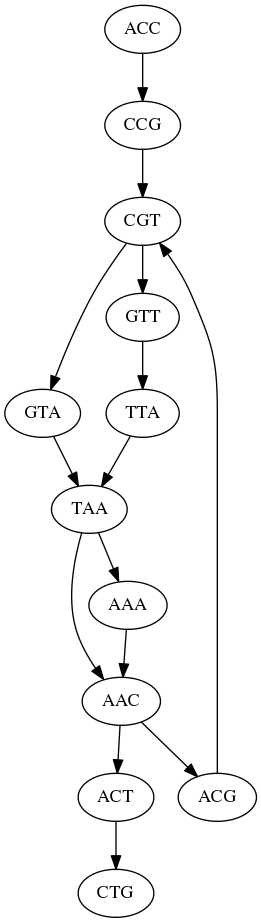
\includegraphics[width=1\textwidth]{deBruijnGraph_4mere.png}
 \caption{De Bruijn graph for the given reads and $k = 4$.}
 \label{fig:4mere}
\end{figure}

\begin{figure}[h]
 \centering
 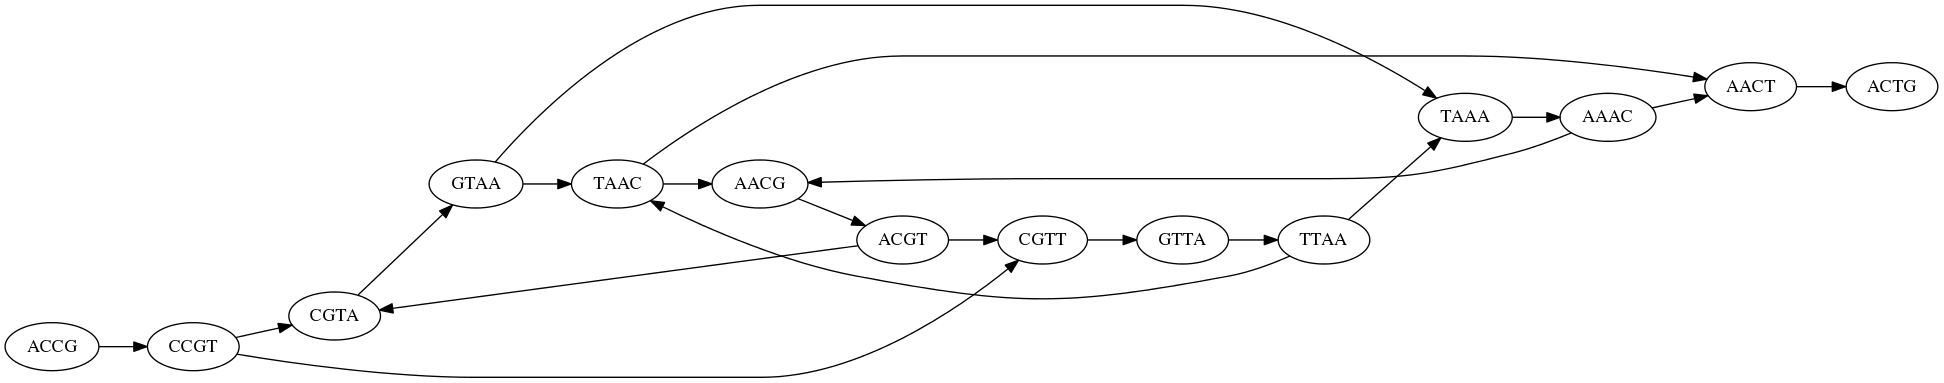
\includegraphics[width=1\textwidth]{deBruijnGraph_5mere.png}
 \caption{De Bruijn graph for the given reads and $k = 5$.}
 \label{fig:5mere}
\end{figure}

\section*{Practical Assignment - \textit{Assemble the human mitochondrial genome}}
\subsubsection*{Introduction}
The mitochondrial genome is rather a small genome in our world. But even this rather small genome, with its $10^4$ basepairs is a though nut, when trying to discover its sequence from reads. For this purpose we used two different alignment algorithms. The Velvet algorithm by Zebrino and Birney is using de Bruijn graphs to assemble the reads.\cite{VelvetProgram}
Likewise does the short oligonucleotide alignment program (SOAP) denovo2 algorithm by Luo et al. use a de Bruijn graph \cite{SOAP2Program}. The differences of both algorithms lie in their detailed structure.\\
The Velvet program starts with building an de Bruijn graph, in which each node has a so called twin node, which represents the reverse complement of the node. Both nodes are called block. The construction of the de Broijn graph happens via two databases. one is a hash table fo r the k-mers, and the second recording the overlaps of the k-mers of a read with other reads. Next a simplification step follows. After this two construction steps, the Error removal starts. The error removing focuses on to three aspects, the removing of tips, bubbles and erroneous connections. There are two rules for tip removing, one is the length is smaller than 2k and the other is called minority count. The minority count is true, if there is an alternative path, which is more common. Bubbles are redundant paths, which are removed via the Tour Bus algorithm. The last correction, removing erroneous connections is based on a threshold which is user set. \cite{VelvetProgram}
The SOAP program is structured in six modules, which handle read error correction, de Bruijn graph construction, contig assembly, paired-end reads mapping, scaffold construction and gap closure. The de Bruijn graph is since SOAPdenovo2 part of the program.\cite{SOAP2Program} Like velvet, does SOAP use a hash table to build up a de Bruijn graph.\cite{SOAP1Program} But before a correction of the sequencing takes place. and afterwards again corrections are applied.

\subsubsection*{Results}
Both algorithms were used to calculate the assembly of the mitochondrial genome separatly. The velvet algorithm was computed on the home source with four different k-mer sizes (from 7 to 31 bases). As a result of the lacking hardware and the missing password for the WSI-Server, the resulting data from the SOAP algorithm was thankfully provided by Sanja Koehlers goup. The statistics for each algorithm are shown in figure \ref{Velvet-Results} and \ref{SOAP-Results}. The for the Velvet program are from the stats.txt and for the SOAP from the XYsoap.contig. The coverage was isolated via a java script (see attachment).

\begin{figure}[h]
	\begin{subfigure}[t] {0.2\textwidth}
	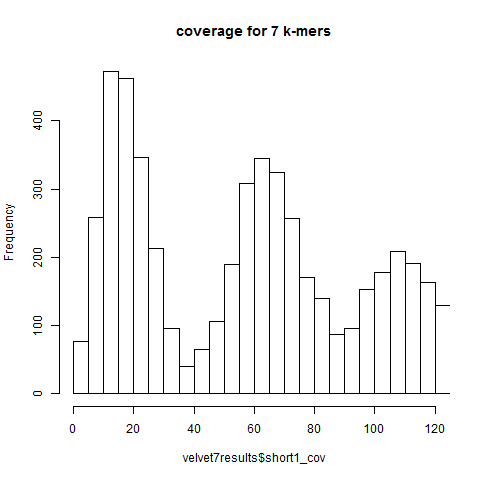
\includegraphics[width=\textwidth]{exercise2/velvet7kmersCoverage.png}
	\caption{k-mer size: 7}
	\label{Velvet-7-mers-coverage}
	\end{subfigure}
	\begin{subfigure}[t] {0.2\textwidth}
		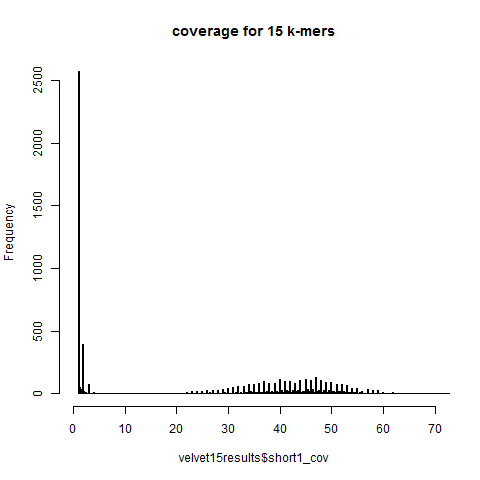
\includegraphics[width=\textwidth]{exercise2/velvet15kmersCoverage.png}
		\caption{k-mer size: 15}
		\label{Velvet-15-mers-coverage}
	\end{subfigure}
	\begin{subfigure}[t] {0.2\textwidth}
		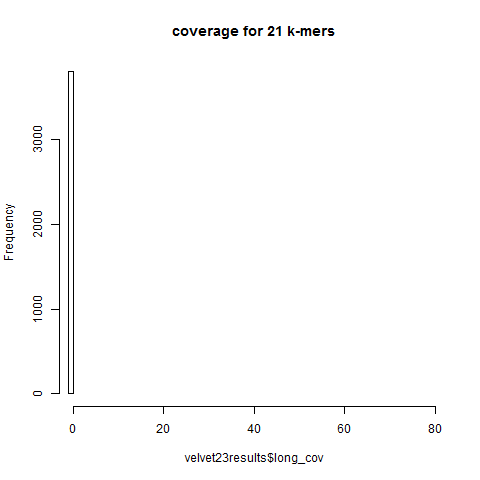
\includegraphics[width=\textwidth]{exercise2/velvet23kmersCoverage.png}
		\caption{k-mer size: 23}
		\label{Velvet-23-mers-coverage}
	\end{subfigure}
	\begin{subfigure}[t] {0.2\textwidth}
		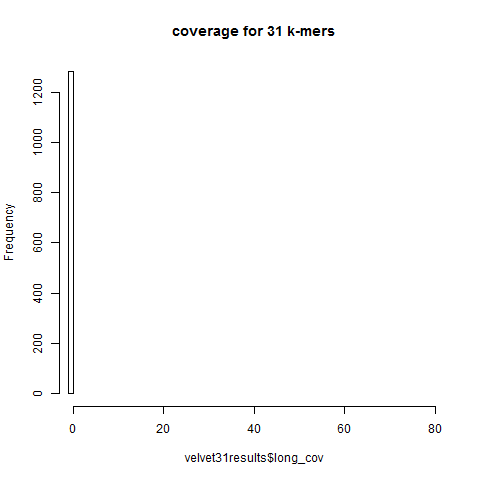
\includegraphics[width=\textwidth]{exercise2/velvet31kmersCoverage.png}
		\caption{k-mer size: 31}
		\label{Velvet-31-mers-coverage}
	\end{subfigure}

	\caption{The figures show the coverage from the Soap program with differing k-mer size for the mitochondrial DNA assembly.}
		\label{Velvet-Results}
\end{figure}

\begin{figure}[h]
	\begin{subfigure}[t] {0.2\textwidth}
		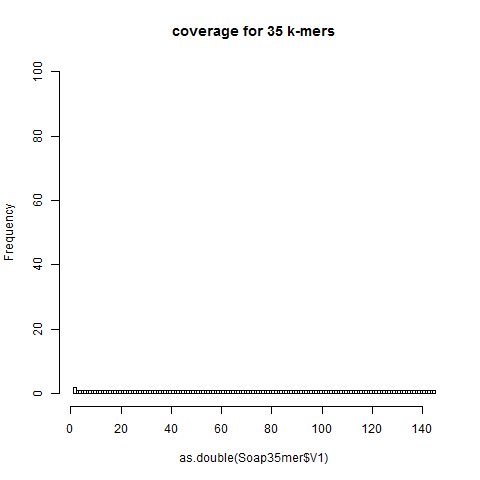
\includegraphics[width=\textwidth]{exercise2/Soap35merCoverage.png}
		\caption{k-mer size: 35}
		\label{SOAP-25-mers-coverage}
	\end{subfigure}
	\begin{subfigure}[t] {0.2\textwidth}
		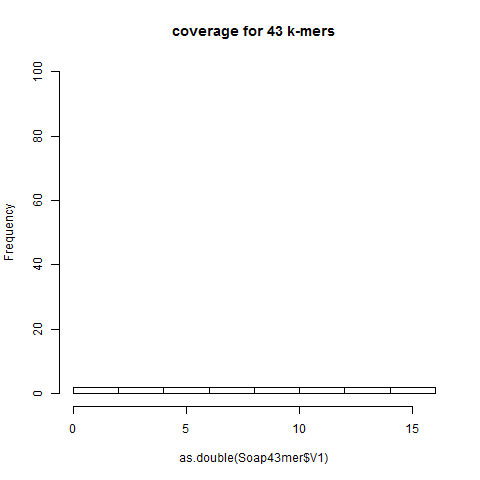
\includegraphics[width=\textwidth]{exercise2/Soap43merCoverage.png}
		\caption{k-mer size: 43}
		\label{SOAP-43-mers-coverage}
	\end{subfigure}
	\begin{subfigure}[t] {0.2\textwidth}
		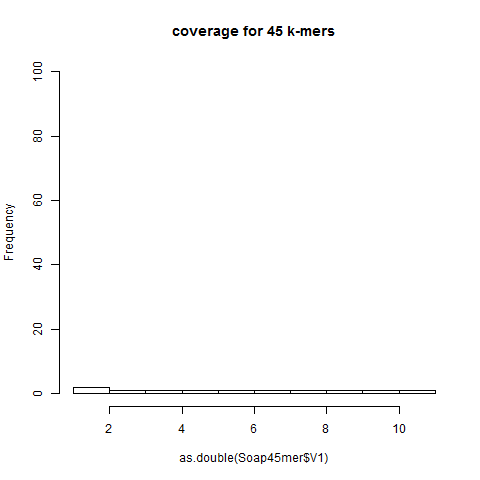
\includegraphics[width=\textwidth]{exercise2/Soap45merCoverage.png}
		\caption{k-mer size: 45}
		\label{SOAP-45-mers-coverage}
	\end{subfigure}
	\begin{subfigure}[t] {0.2\textwidth}
		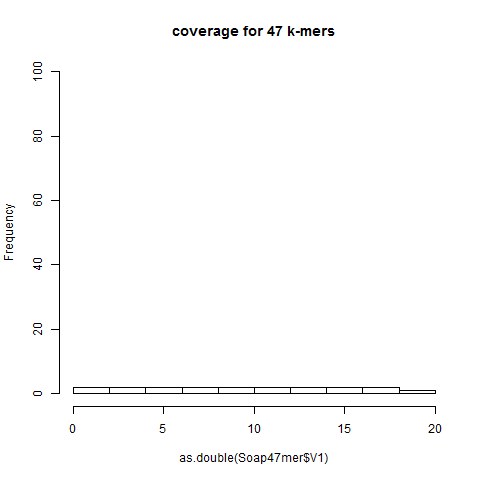
\includegraphics[width=\textwidth]{exercise2/Soap47merCoverage.png}
		\caption{k-mer size: 47}
		\label{SOAP-47-mers-coverage}
	\end{subfigure}

	\caption{The figures show the coverage from the Soap program with differing k-mer size for the mitochondrial DNA assembly.}
		\label{SOAP-Results}
\end{figure}

\subsubsection*{Discussion}
The smaller the k-mer the more contigs are the result as it is visible in figure \ref{Velvet-7-mers-coverage}. Larger k-mers have as result more unique contigs \cite{VelvetProgram}. Generally we can not conclude anything from our results for the quality of the algorithms, because we did not use the same k-mer length. But an optimal k-mer size is a compromise between uniqueness of the k-mer (longer) and resulting amount of contigs (shorter).

\subsubsection*{Acknowledgement}
Thanks again to Sanja Koehler an her group for the SOAP-data.

\begin{thebibliography}{20}
	\bibitem{VelvetProgram} Velvet: algorithms for de novo short read assembly using de Bruijn graphs. D.R. Zerbino and E. Birney. Genome Research 18:821-829. 
	\bibitem{SOAP2Program} SOAPdenovo2: an empirically improved memory-efficient short-read de novo assembler. Luo et al. GigaScience 2012 1:18.
	\bibitem{SOAP1Program}SOAP: short oligonucleotide alignment program" (2008) BIOINFORMATICS,Vol. 24 no.5 2008, pages 713–714 doi:10.1093/bioinformatics/btn025
	
\end{thebibliography}



\end{document}